% ---------------------------------------------------------------------------
% Author guideline and sample document for EG publication using LaTeX2e input
% D.Fellner, v2, June 1, 2017

\documentclass{egpubl}

% --- for  Annual CONFERENCE
% \ConferenceSubmission % uncomment for Conference submission
% \ConferencePaper      % uncomment for (final) Conference Paper
% \STAR                 % uncomment for STAR contribution
% \Tutorial             % uncomment for Tutorial contribution
% \ShortPresentation    % uncomment for (final) Short Conference Presentation
%
% --- for  CGF Journal
% \JournalSubmission    % uncomment for submission to Computer Graphics Forum
 \JournalPaper         % uncomment for final version of Journal Paper
%
% --- for  CGF Journal: special issue
% \SpecialIssueSubmission    % uncomment for submission to Computer Graphics Forum, special issue
% \SpecialIssuePaper         % uncomment for final version of Journal Paper, special issue
%
% --- for  EG Workshop Proceedings
% \WsSubmission    % uncomment for submission to EG Workshop
% \WsPaper         % uncomment for final version of EG Workshop contribution
%
 \electronicVersion % can be used both for the printed and electronic version

% !! *please* don't change anything above
% !! unless you REALLY know what you are doing
% ------------------------------------------------------------------------

% for including postscript figures
% mind: package option 'draft' will replace PS figure by a filname within a frame
\ifpdf \usepackage[pdftex]{graphicx} \pdfcompresslevel=9
\else \usepackage[dvips]{graphicx} \fi

\PrintedOrElectronic

% prepare for electronic version of your document
\usepackage{t1enc,dfadobe}

\usepackage{egweblnk}
\usepackage{cite}
\usepackage[utf8]{inputenc}
\usepackage{listings}
% For backwards compatibility to old LaTeX type font selection.
% Uncomment if your document adheres to LaTeX2e recommendations.
% \let\rm=\rmfamily    \let\sf=\sffamily    \let\tt=\ttfamily
% \let\it=\itshape     \let\sl=\slshape     \let\sc=\scshape
% \let\bf=\bfseries

% end of prologue
% ---------------------------------------------------------------------
% EG author guidelines plus sample file for EG publication using LaTeX2e input
% D.Fellner, v2.02, Jan 25, 2017
% CONTENT HERE ON...

\title[Natural neighbor interpolation of images and volumes]%
{Natural neighbor interpolation of images and volumes}

% for anonymous conference submission please enter your SUBMISSION ID
% instead of the author's name (and leave the affiliation blank) !!
\author[Jan Živković]
{\parbox{\textwidth}{\centering Jan Živković}
	\\
	{\parbox{\textwidth}{\centering Univerza v Ljubljani Fakulteta za računalništvo in informatiko, Slovenia}
	}
}
% ------------------------------------------------------------------------

% if the Editors-in-Chief have given you the data, you may uncomment
% the following five lines and insert it here
%
% \volume{36}   % the volume in which the issue will be published;
% \issue{1}     % the issue number of the publication
% \pStartPage{1}      % set starting page


%-------------------------------------------------------------------------
\begin{document}
	
	% uncomment for using teaser
	% \teaser{
	%  \includegraphics[width=\linewidth]{eg_new}
	%  \centering
	%   \caption{New EG Logo}
	% \label{fig:teaser}
	%}
	
	\maketitle
	%-------------------------------------------------------------------------
	\begin{abstract}
		V seminarski nalogi se prikaže način generiranja slike z le nekaj vzorci točk in pripadajočo barvo na teh točkah. Glede na te podatke se zgenerira voronoi graf in nato za vsako pixel slike izračuna barva, da se lahko nato izriše slika, ki je bila zgenerirana s podanimi podatki. Slika je z majhnim številom vzorcev bolj 'zamegljena', z večjim številom vzorcev pa je vedno bolj podobna originalu. Opisana je samo 2D implementacija z optimizacijami, 3D implementacije pa ni implementirane.
		%-------------------------------------------------------------------------
		%  ACM CCS 1998
		%  (see http://www.acm.org/about/class/1998)
		% \begin{classification} % according to http:http://www.acm.org/about/class/1998
		% \CCScat{Computer Graphics}{I.3.3}{Picture/Image Generation}{Line and curve generation}
		% \end{classification}
		%-------------------------------------------------------------------------
		%  ACM CCS 2012
		%The tool at \url{http://dl.acm.org/ccs.cfm} can be used to generate
		% CCS codes.
		%Example:
		  
	\end{abstract}  
	%-------------------------------------------------------------------------
	\section{Uvod}
	
	V seminarski nalogi je predstavljen način za naravno interpolacijo sosedov v 2D prostoru z slikami in 3D prostoru u volumni. S tem lahko z nekaj vzorci barv in lokacijo tega vzorca(x, y v 2D in x, y, z v 3D) preračunamo barvo z naravno interpolacijo.
	
	%-------------------------------------------------------------------------
	\section{Voronoi graf}\label{voronoi}
	Na začetku potrebujemo voronoi graf, ki ga zgeneriramo s pomočjo paketa scipy. Grafu se poda vzorčne točke, iz katerih nato izračuna voronoi regije. Primer voronoi grafa z neskončnimi robovi je prikazan na sliki \ref{fig:voronoi_inf_edges}.
	
	\begin{figure}[htb]
		\centering
		\parbox[t]{.9\columnwidth}{\relax
			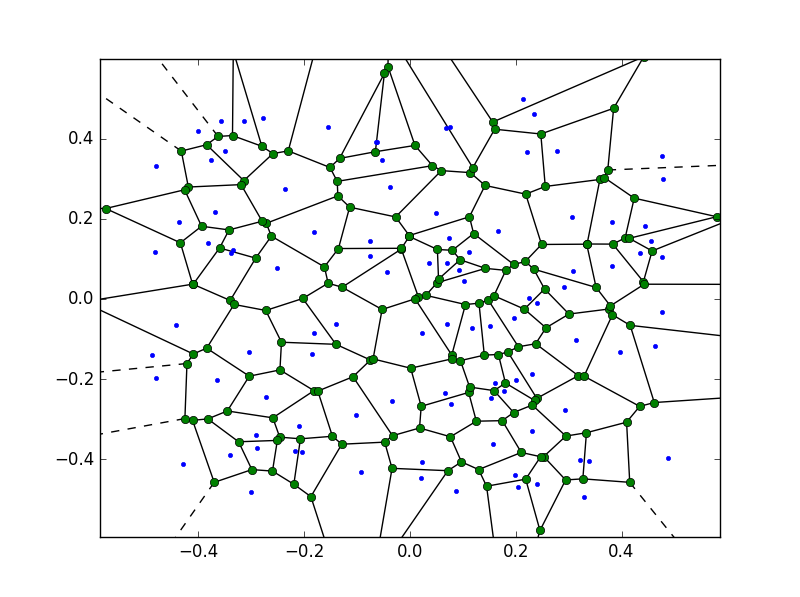
\includegraphics[width=.95\linewidth]{voronoi_inf.png}
		}
		\caption{\label{fig:voronoi_inf_edges}
			Voronoi graf z neskončnimi robovi.}
	\end{figure}
	
	\subsection{Omejevanje grafa v 2D prostoru}
	V 2D implementaciji je bil problem, da je generirana slika imela črne robove, kjer je voronoi graf izračunal regije z neskončnimi robovi, kot je to razvidno na sliki \ref{fig:voronoi_inf_edges}. Zaradi tega je izračun barve vrnil črno barvo. Primer zgenerirane slike s črnimi robovi je na sliki \ref{fig:black_edges}.
	
	\begin{figure}[htb]
		\centering
		\parbox[t]{.9\columnwidth}{\relax
			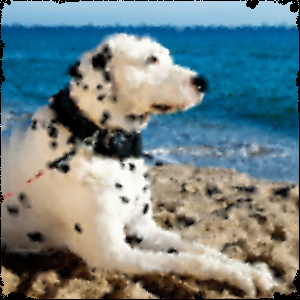
\includegraphics[width=.95\linewidth]{300x300x10000_black_edges.png}
		}
		\caption{\label{fig:black_edges}
			300x300 slika z 10000 vzorci s črnimi robovi.}
	\end{figure}
	
	Graf je bilo potrebno torej omejiti, oziroma zgenerirati tako, da so vse točke, ki se nahajajo na sliki v zaprtih voronoi regijah in ne odprtih. Na začetku je bila ideja da ročno dodamo dodatne točke izven velikosti slike, a se ta način ni obnesel. Kasneje sem našel boljši način na 'stackoverflow', ki vzorčne točke preslika čez meje slike, torej če je slika velikosti 300x300, preslika točke v 4 smeri:
		\begin{itemize} 
		\item preslika vse originalne vzorčne točke čez x=0
		\item preslika vse originalne vzorčne točke čez x=300
		\item preslika vse originalne vzorčne točke čez y=0
		\item preslika vse originalne vzorčne točke čez y=300
	\end{itemize}
	
	Primer zgeneriranega voronoi grafa s preslikanimi točkami je na sliki \ref{fig:clipped_voronoi}. S tem se število točk s katerimi se izračuna voronoi graf poveča za 5x, kot tudi čas izračuna grafa, a je le ta dokaj zanemarljiv(kot če bi sami med izvajanjem omejevali graf). 
	
	\begin{figure}[htb]
		\centering
		\parbox[t]{.9\columnwidth}{\relax
			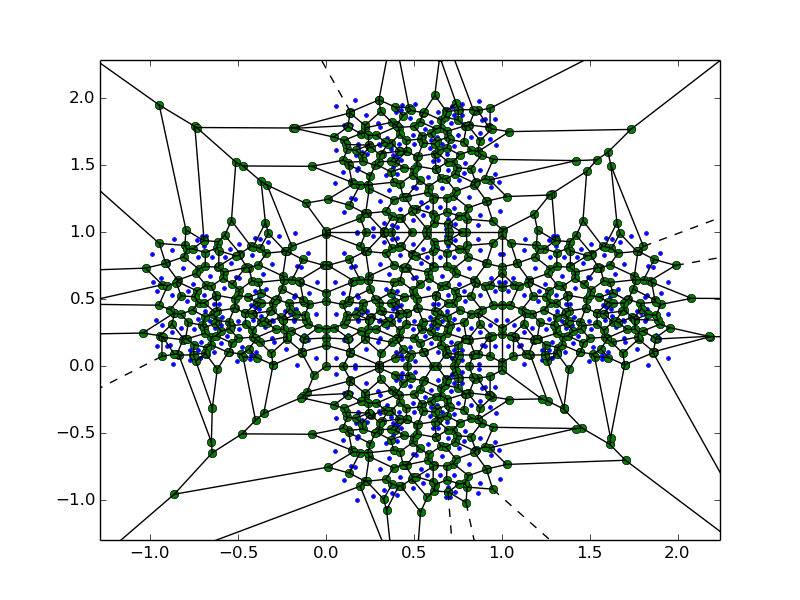
\includegraphics[width=.95\linewidth]{bounded_voronoi.png}
		}
		\caption{\label{fig:clipped_voronoi}
			Omejen voronoi graf s preslikanimi točkami.}
	\end{figure}

	\begin{figure}[htb]
		\centering
		\parbox[t]{.9\columnwidth}{\relax
			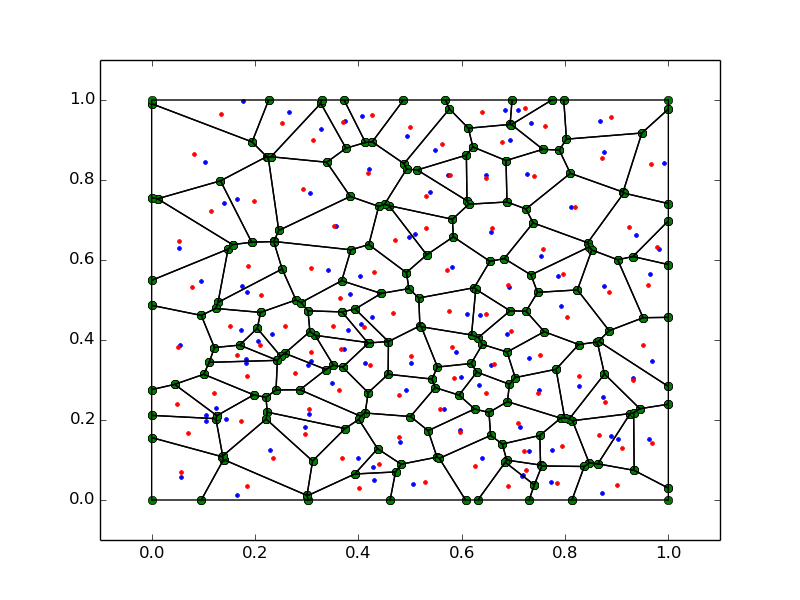
\includegraphics[width=.95\linewidth]{voronoi.png}
		}
		\caption{\label{fig:voronoi}
			Voronoi graf z omejenimi robovi.}
	\end{figure}
	
	\subsection{Omejevanje grafa v 3D prostoru}
	Po vsem raziskovanju, bi na isti problem kot na 2D naletel tudi pri 3D, le da bi tukaj moral preslikati točke čez vse ploskve volumna(oziroma čez bounding box volumna).
	
	%-------------------------------------------------------------------------
	\section{Implementacija}
	
	V sklopu seminarske naloge je potrebno implementirati 2D in 3D implementacijo. Tu je opisana in narejena le 2D implementacija, saj mi 3D ni uspelo implementirati.
	
	\subsection{2D}
	Implementacijo sem izdelal v programskem jeziku Python3, za kar sem se odločil zato, ker ima že pakete za generacijo voronoi grafov, kot tudi za KDTree in olajša delo z algoritmi. Nekaj kode je tudi napisane v jeziku Cython \cite{cython}, ki je kombinacija jezika Python in C, s čimer sem lahko pohitril dele kode.
	
	Implementacijo sem začel z uporabo voronoi grafa, ki je opisan v \ref{voronoi} točki. Na začetku se z omejevanjem voronoi grafa nisem ukvarjal in sem le to pustil za zadnjo stvar. Ko sem imel voronoi graf izračunan sem začel z implementacijo funkcije za dodajanje točke v graf(prikazan v izseku kode \ref{lst:add_point}).
	Algoritem deluje tako, da poišče najbližjo točko vstavljeni točki, nato izračuna pravokotni bisektor in najde robova(od regije najbližje točke), ki ju pravokotni bisektor seka. Pridobljena robova morata biti sortirana 'ccw'(s čimer povemo da generiramo robove vstavljene točke v nasprotni smeri urinega kazalca). Rob dobimo z kreiranjem črte, ki gre od točke kjer je sekan prvi rob, do točke kjer je sekan drugi rob. Sedaj ko imamo rob vstavljene točke, lahko izračunamo ploščino poligona, ki smo ga 'ukradli' najbližji točki. Ploščino bomo kasneje uporabili za izračun barve. Ta proces ponavljamo dokler ne zgeneriramo roba, ki robove sklene v zanko. Ko imamo zgeneriran celotni poligon, lahko izračunamo barvo vstavljene točke in le to vrnemo. Ta postopek se ponavlja toliko časa dokler ne izračunamo barve vseh pixlov slike. Na sliki \ref{fig:insert_point} se vidi kako se izračuna ukraden voronoi poligon.
	
	Pseudokoda algoritma je:
	\begin{lstlisting}[language=Python,basicstyle=\tiny, caption={Pseudokoda algoritma za izračun barve točke},captionpos=b,label={lst:add_point}]
def add_point(self, point):
	list_of_area_and_color = []
	closest_point = self.get_closest_point(point)
	perpendicular_bisector = self.get_perpendicular_bisector(
		closest_point['point'], point
	)
	e1, e2 = self.get_edges_crossing_bisector(
		closest_point, perpendicular_bisector, point
	)
	list_of_area_and_color.append(
		self.calculate_area_taken((e1, e2), closest_point)
	)
	
	final_edge = e1
	prev_point = closest_point
	loop_counter = 0
	while not self.edge_equals(e2, final_edge):
		if loop_counter > 20: return 0
		other_point = self.get_other_point(e2, prev_point)
		perpendicular_bisector = self.get_perpendicular_bisector(
			other_point['point'], point
		)
		e1, e2 = self.get_edges_crossing_bisector(
			other_point, perpendicular_bisector, point
		)

		list_of_area_and_color.append(
			self.calculate_area_taken((e1, e2), other_point)
		)
		prev_point = other_point
		loop_counter += 1
	
	return self.calculate_weighed_color(list_of_area_and_color)
	\end{lstlisting}
	
	\begin{figure}[!htb]
		\centering
		\parbox[t]{.7\columnwidth}{\relax
			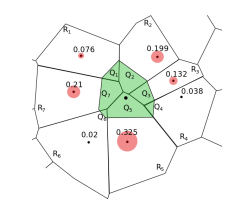
\includegraphics[width=.95\linewidth]{insert_point.png}
		}
		\caption{\label{fig:insert_point}
			Primer izračuna nove voronoi regije za vstavljeno točko.}
	\end{figure}
	
	\subsubsection{Izračun barve za točko}
	Med izračunom regije za vstavljeno točko si tudi shranim barvo točke kateri sem 'ukradel' kos regije in pa samo ploščino ukradenega kosa regije.
	Nato se barva izračuna glede na procent ukradene ploščine poligona glede na celotno ploščino ukradenega poligona vstavljene točke. V izseku kode \ref{lst:calculate_weighed_color} je prikazana pseudokoda za izračun barve.
	
	\begin{lstlisting}[language=Python,basicstyle=\tiny, caption={Pseudokoda algoritma za izračun barve točke},captionpos=b,label={lst:calculate_weighed_color}]
def calculate_weighed_color(list list_area_and_color not None, int n):
	cdef double full_area = 0
	cdef int i
	for i in range(n):
		full_area += list_area_and_color[i][0]
	cdef int r = 0, g = 0, b = 0
	cdef list t
	for i in range(n):
		t = list_area_and_color[i]
		percentage = t[0] / full_area
		r += t[1][0] * percentage
		g += t[1][1] * percentage
		b += t[1][2] * percentage
	cdef double output[3]
	output[0] = round(r)
	output[1] = round(g)
	output[2] = round(b)
	return output
	\end{lstlisting}
	
	Za izračun barve sem uporabil drugačen algoritem, kot je opisano v \cite{algorithm} z namenom hitrejšega izračuna, saj ni potrebno izračunati ploščine za vse regije vzorčnih točk. Razlika v izračunani barvi je minimalna in s prostim očesom neopazna, zato sem se odločil da uporabim svoj algoritem.

	\subsubsection{Optimizacije}
	V nalogi sem uporabil razne optimizacije, da bi program deloval kar se da hitro. Te optimizacije so naštete spodaj:
	
	\begin{itemize} 
		\item[--]  Vračanje barve za točko, če je le ta točka ena izmed vzorčenih točk
		\item[--] cKDTree (namesto naivne funkcije, ki gre čez vse točke da najde najbližjo točko iskani točki)
		\item[--] Memoizacija (memoizacija funkcije za vračanje robov voronoi regije)
		\item[--] Cython (optimizacija določenih funkcij z izvajanjem kode v C jeziku)
	\end{itemize}
	
	\noindent
	Funkcije optimizirane z Cython:
	\begin{itemize} 
		\item[--] get\_line\_intersection (največja optimizacija, iz 20 sekund na 0.7 sekunde pri 300x300 sliki z 10000 vzorčnimi točkami)
		\item[--] ccw
		\item[--] get\_center\_on\_line
		\item[--] get\_perpendicular\_bisector
		\item[--] calculate\_area\_from\_vertices
		\item[--] calculate\_weighed\_color
		\item[--] calculate\_area\_for\_stolen\_polygon
	\end{itemize}

	Vse optimizirane funkcije se nahajajo v datoteki 'optimized.pyx'. Za uporabo Cython kode je bilo potrebno namestiti razvojna orodja za Python in razvojna orodja za C/C++ jezik. Optimizirane funkcije se s Cython prevedejo v C kodo, katera se nato prevede v C program, ki ga Cython v Python kodo doda kot Python paket. Uporaba zgoraj naštetih optimizacij je izvajanje programa zmanjšala z približno 180 sekund na 'le' 21 sekund.
	
	Nadaljne optimizacije bi lahko bile, da se program izvaja na grafični kartici z CUDA ali PYOpenCL vendar bi to potrebovalo prepis in reorganizacijo celotne kode, kot tudi veliko časa in potrpljenja.
	
	\subsubsection{Primeri izračunanih slik}
	Tu je prikazan primer izračunane slike z podano vhodno sliko.
	
	\begin{figure}[!htb]
		\centering
		\parbox[t]{.7\columnwidth}{\relax
			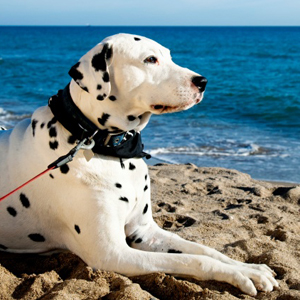
\includegraphics[width=.95\linewidth]{300x300.jpg}
		}
		\caption{\label{fig:300x300_source}
			300x300 slika na podlagi katere se izračunava.}
	\end{figure}

	\begin{figure}[!htb]
		\centering
		\parbox[t]{.7\columnwidth}{\relax
			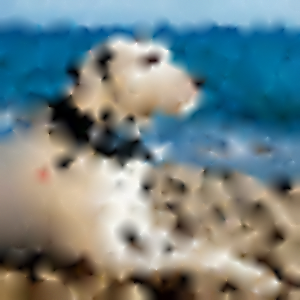
\includegraphics[width=.95\linewidth]{300x300x1000_result.png}
		}
		\caption{\label{fig:300x300x1000}
			300x300 slika narejena z 1000 vzorčnimi točkami.}
	\end{figure}

	\begin{figure}[!htb]
		\centering
		\parbox[t]{.7\columnwidth}{\relax
			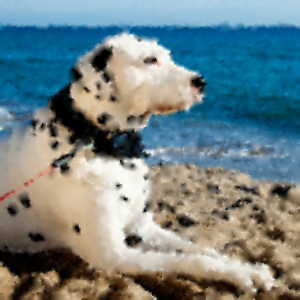
\includegraphics[width=.95\linewidth]{300x300x10000_result.png}
		}
		\caption{\label{fig:300x300x10000}
			300x300 slika narejena z 10000 vzorčnimi točkami.}
	\end{figure}


	\begin{figure}[!htb]
		\centering
		\parbox[t]{.75\columnwidth}{\relax
			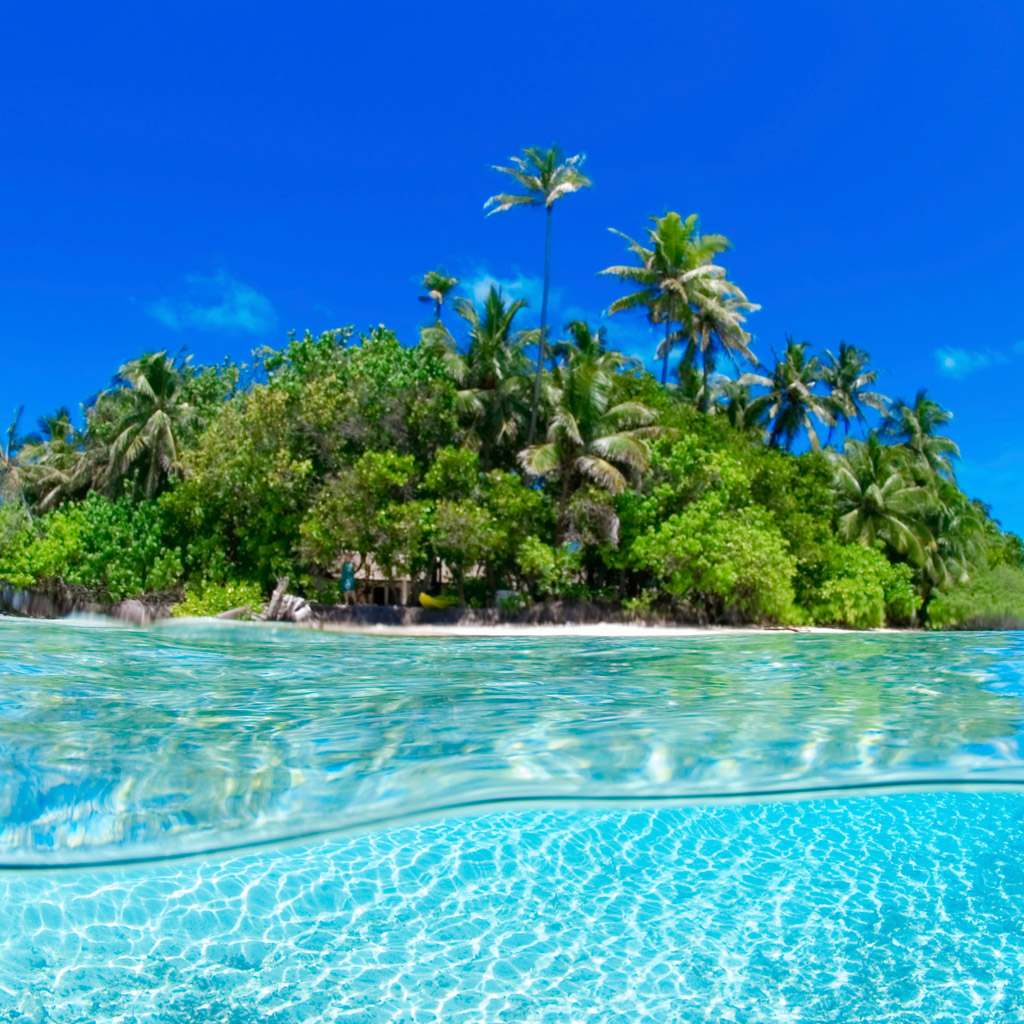
\includegraphics[width=.95\linewidth]{1024x1024.jpg}
		}
		\caption{\label{fig:1024x1024_source}
			1024x1024 slika na podlagi katere se izračunava.}
	\end{figure}
	
	\begin{figure}[!htb]
		\centering
		\parbox[t]{.75\columnwidth}{\relax
			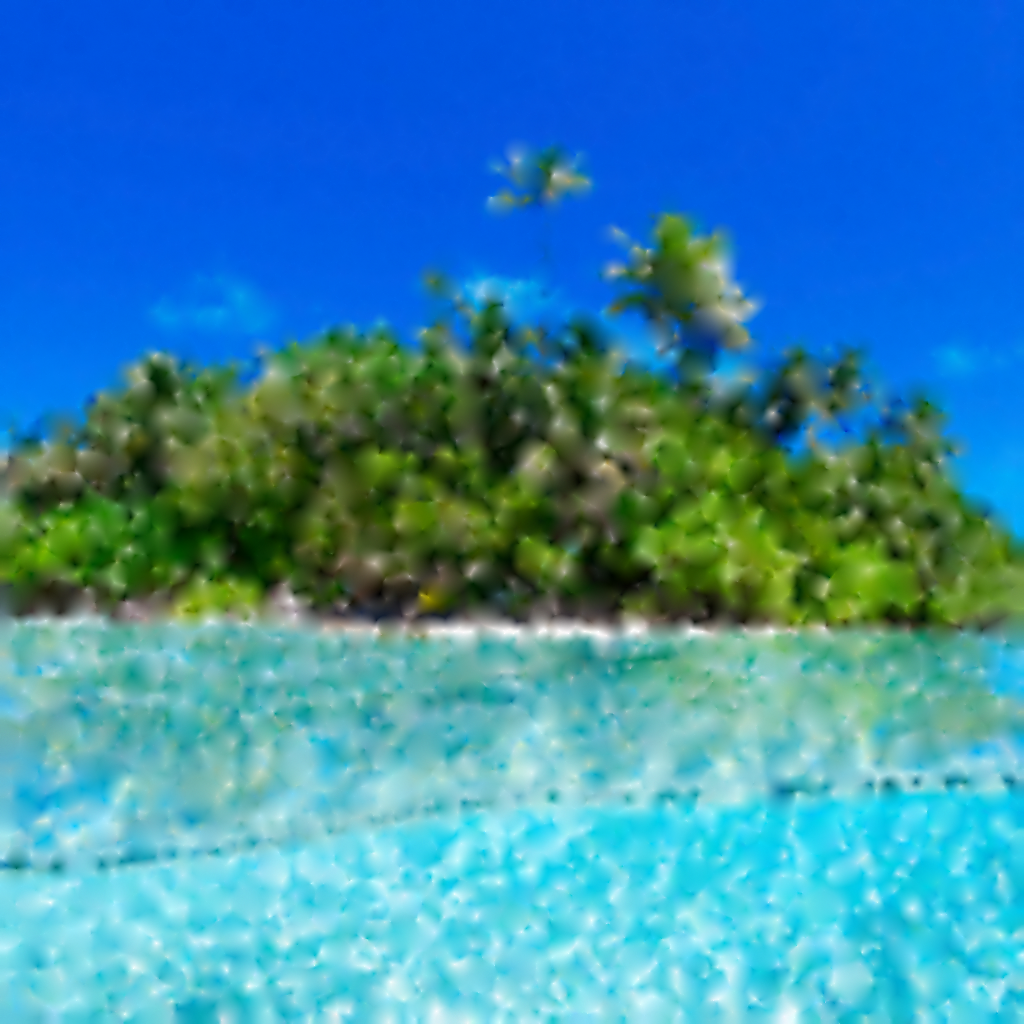
\includegraphics[width=.95\linewidth]{1024x1024x10000_result.png}
		}
		\caption{\label{fig:1024x1024x10000}
			1024x1024 slika narejena z 10000 vzorčnimi točkami.}
	\end{figure}
	
	\begin{figure}[!htb]
		\centering
		\parbox[t]{.75\columnwidth}{\relax
			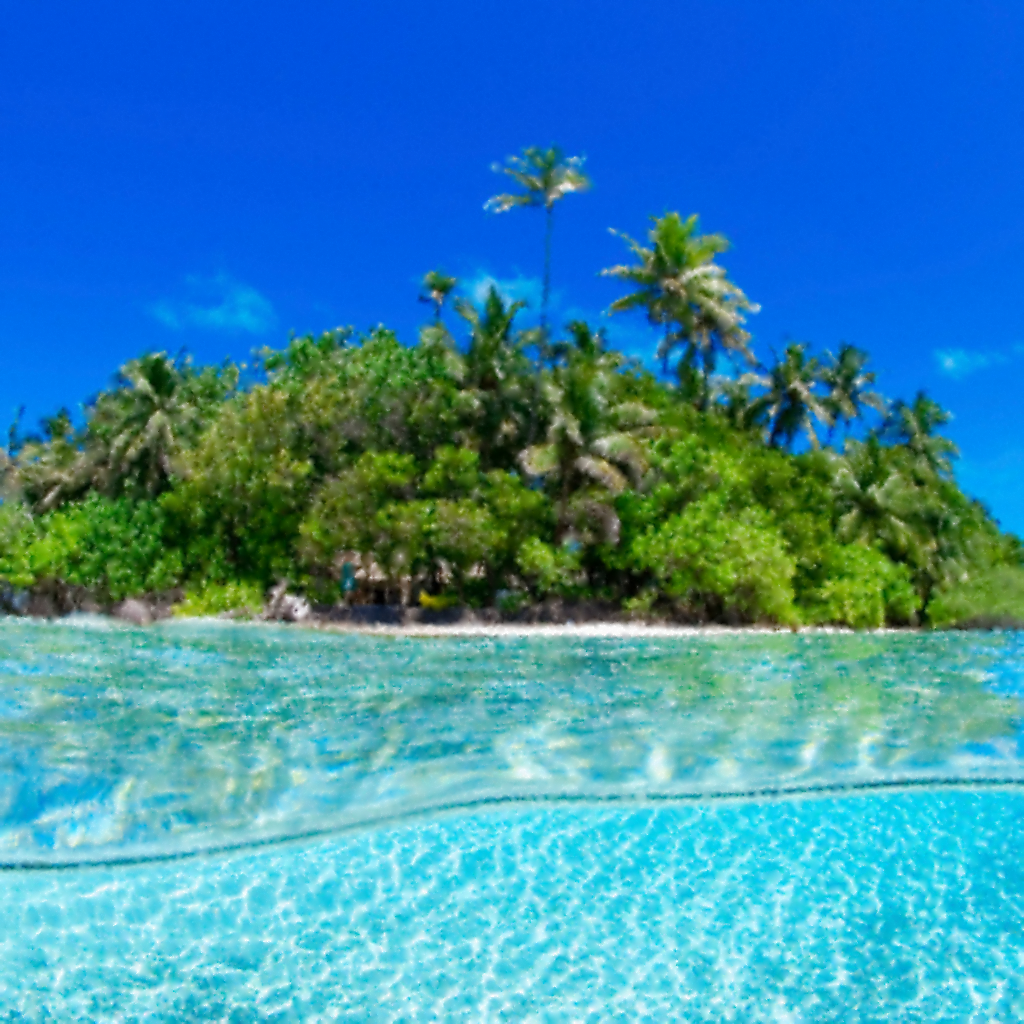
\includegraphics[width=.95\linewidth]{1024x1024x100000_result.png}
		}
		\caption{\label{fig:1024x1024x100000}
			1024x1024 slika narejena z 100000 vzorčnimi točkami.}
	\end{figure}


	\subsection{3D}
	3D implementacija ni narejena, a bi po vsej verjetnosti bila narejena na isti način kot 2D, z razlikami kako bi sortirali točke in robove, namesto voronoi regij bi uporabljali voronoi poligone itd. To implementacijo bi bilo skoraj nujno implementirati na grafični kartici, saj bi se ta na procesorju izračunavala veliko počasneje.
	
	\section{Zaključek}
	Sama seminarska naloga je bila zelo zanimiva, celo bolj kot sem pričakoval. Implementacija naloge mi je vzela veliko časa, vmes sem imel veliko problemov, kot so recimo:
	\begin{itemize}
		\item napačno generiranje regije za vstavljeno točko v določenih primerih
		\item napačen izračun ploščine ukradenega poligona(včasih je izračunal ukraden kos poligona, včasih pa preostal kos poligona)
		\item napačen izračun barve(overflow modre barve v zeleno zaradi uporabe integer zapisa barve) 
	\end{itemize}

	Samo debugiranje kode je bilo dokaj zahtevno, saj je do problema ponavadi prišlo globoko med izvajanjem, zato sem si ustvaril datoteko, kjer sem lahko imel vedno iste podatke za generiranje slike, jo naložil v program in tako vedno izvajal vstavljenje točke na kontroliranih podatkih, si izrisoval grafe in lažje našel napako.
	
	Vsa izvorna koda celotnega seminarja je na voljo na spletnem naslovu \cite{source_code}.
	
	\bibliographystyle{eg-alpha-doi}
	\bibliography{literatura}
	
\end{document}

